\chapter{Linear classification: Support Vector Machine, Softmax}
\section{Linear Classification}
Disadvantages of kNN
\begin{itemize}
  \item The classifier must remember all of the training data and store it for future comparisons with the test data: this is space inefficient because datasets may easily be gigabytes in size.
  \item Classifying a test image is expensive since it requires a comparison to all training images.
\end{itemize}

New approach with two major components:
\begin{itemize}
  \item \textbf{Score function}: maps the raw data to class scores.
  \item \textbf{Loss function}: quantifies the agreement between the predicted scores and the ground truth labels.
\end{itemize}

\textbf{Goal}: minimize the loss function with respect to the parameters of the score function. 

\section{Parameterized mapping from images to label scores}
\textbf{Score function}: maps the pixel values of an image to confidence scores for each class. 

For example, let�s assume a training dataset of images $x_i\in R^D$, each associated with a label $y_i$. 
Here $i=1,\ldots, N_i$ and $y_i\in 1,\ldots, K$. 
That is, we have $N$ examples (each with a dimensionality $D$) and $K$ distinct categories. 
For example, in CIFAR-10 we have a training set of $N = 50,000$ images, each with $D = 32 \times 32 \times 3 = 3072$ pixels, and $K = 10$, since there are 10 distinct classes (dog, cat, car, etc). 
We will now define the score function $f:R^D\rightarrow R^K$ that maps the raw image pixels to class scores. 

\subsection{Linear classifier.}
Let's start out with arguably the simplest possible function, a linear mapping:
$$f(x_i,W,b)=Wx_i+b$$
\begin{itemize}
  \item Assume image $x_i$ has all of its pixels flattened out to a single column vector of shape $[D \times 1]$.
  \item $W$: \textbf{Weights} (of size $[K \times D]$).
  \item $b$: \textbf{bias vector} (of size $[K x 1]$) - it influences the output scores, but without interacting with the actual data $x_i$
\end{itemize}

\textbf{Remark}:
\begin{itemize}
  \item The single matrix multiplication $Wx_i$ is effectively evaluating 10 separate classifiers in parallel (one for each class), where each classifier is a row of $W$.
  \item The input data $(x_i,y_i)$ as given and fixed, but we have control over the setting of the parameters $W$, $b$. Our goal will be to set these in such way that the computed scores match the ground truth labels across the whole training set.
  \item An advantage of this approach is that the training data is used to learn the parameters $W$, $b$, but once the learning is complete we can discard the entire training set and only keep the learned parameters.
  \item To classifying the test image involves a single matrix multiplication and addition, which is significantly faster than comparing a test image to all training images.
\end{itemize}

\begin{figure}[ht]
  \centering
  % Requires \usepackage{graphicx}
  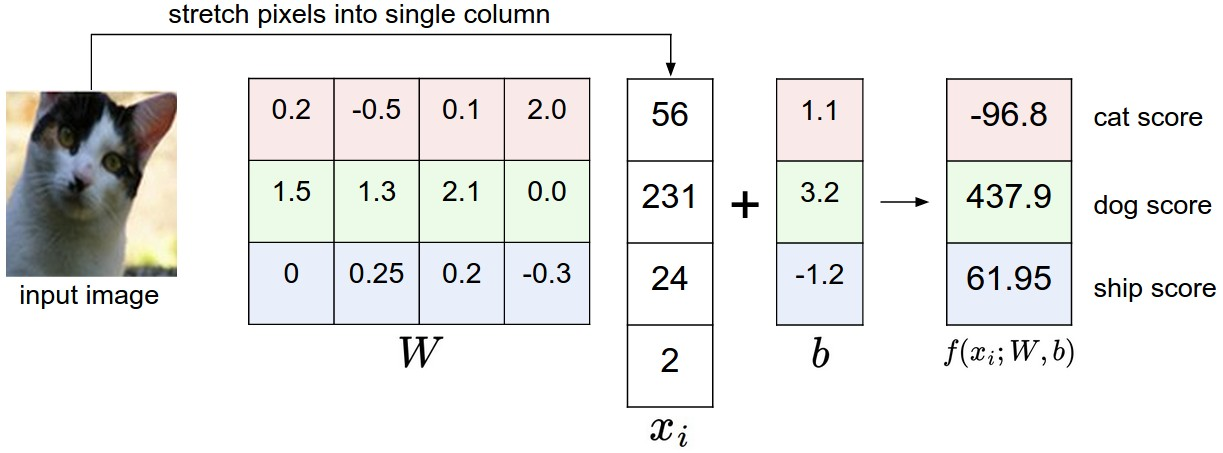
\includegraphics[width=5 in]{pic/imagemap}\\
  \caption{An example of mapping an image to class scores. For the sake of visualization, we assume the image only has 4 pixels (4 monochrome pixels, we are not considering color channels in this example for brevity), and that we have 3 classes (red (cat), green (dog), blue (ship) class). (Clarification: in particular, the colors here simply indicate 3 classes and are not related to the RGB channels.) We stretch the image pixels into a column and perform matrix multiplication to get the scores for each class. Note that this particular set of weights W is not good at all: the weights assign our cat image a very low cat score. In particular, this set of weights seems convinced that it's looking at a dog.}
\end{figure}

\subsection{Analogy of images as high-dimensional points.}
\begin{figure}[ht]
  \centering
  % Requires \usepackage{graphicx}
  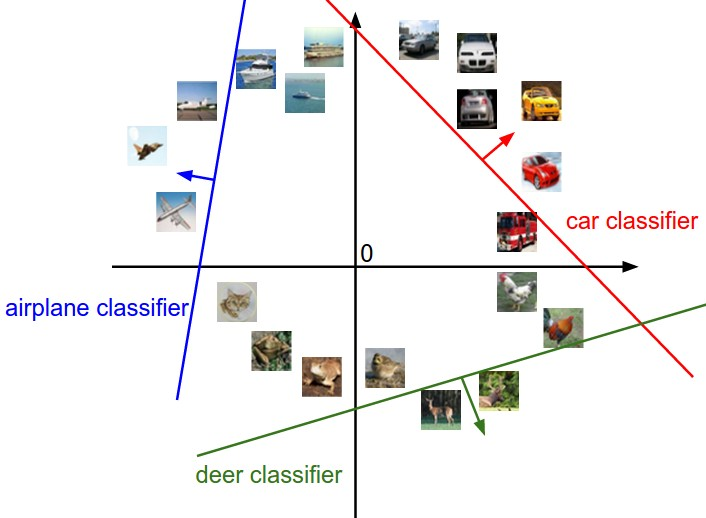
\includegraphics[width=5 in]{pic/pixelspace}\\
  \caption{Every row of $W$ is a classifier for one of the classes. The geometric interpretation of these numbers is that as we change one of the rows of $W$, the corresponding line in the pixel space will rotate in different directions. The biases $b$ allow our classifiers to translate the lines. In particular, note that without the bias terms, plugging in $x_i=0$ would always give score of zero regardless of the weights, so all lines would be forced to cross the origin.}
\end{figure}

\subsection{Interpretation of linear classifiers as template matching.}
Another interpretation for the weights WW is that each row of WW corresponds to a template (or sometimes also called a prototype) for one of the classes. The score of each class for an image is then obtained by comparing each template with the image using an inner product (or dot product) one by one to find the one that �fits� best. With this terminology, the linear classifier is doing template matching, where the templates are learned. Another way to think of it is that we are still effectively doing Nearest Neighbor, but instead of having thousands of training images we are only using a single image per class (although we will learn it, and it does not necessarily have to be one of the images in the training set), and we use the (negative) inner product as the distance instead of the L1 or L2 distance.


